%% 
%% Copyright 2019-2024 Elsevier Ltd
%% 
%% Version 2.4
%% 
%% This file is part of the 'CAS Bundle'.
%% --------------------------------------
%% 
%% It may be distributed under the conditions of the LaTeX Project Public
%% License, either version 1.2 of this license or (at your option) any
%% later version.  The latest version of this license is in
%%    http://www.latex-project.org/lppl.txt
%% and version 1.2 or later is part of all distributions of LaTeX
%% version 1999/12/01 or later.
%% 
%% The list of all files belonging to the 'CAS Bundle' is
%% given in the file `manifest.txt'.
%% 
%% Template article for cas-sc documentclass for 
%% single column output.

%\documentclass[a4paper,fleqn,longmktitle]{cas-sc}
\documentclass[a4paper,fleqn]{cas-sc}

\usepackage[numbers]{natbib}
%\usepackage[authoryear]{natbib}
% \usepackage[authoryear,longnamesfirst]{natbib}
\usepackage{fvextra}
\usepackage{tabularray}
\usepackage{float}

% % remove left footer
% \usepackage{fancyhdr} % Ensure this is included (usually already in Elsevier templates)
% \pagestyle{fancy}     % Use the fancy page style
% \lfoot{}              % Clear the left footer

%%%Author macros
\def\tsc#1{\csdef{#1}{\textsc{\lowercase{#1}}\xspace}}
\tsc{WGM}
\tsc{QE}
\tsc{EP}
% \tscawew{PMS}
\tsc{BEC}
\tsc{DE}
%%%

\begin{document}
\let\WriteBookmarks\relax
\def\floatpagepagefraction{1}
\def\textpagefraction{.001}

\shorttitle{A Meta-learning approach in movement prediction of aperiodic time-series data}
\shortauthors{B.L. Nguyen et~al.}

%\begin{frontmatter}

\title [mode = title]{A Meta-learning approach in movement prediction of aperiodic time-series data}
\tnotemark[1]

\tnotetext[1]{This research did not receive any specific grant from funding agencies in the public, commercial, or not-for-profit sectors.}

% % \tnotetext[2]{The second title footnote which is a longer text matter to fill through the whole text width and overflow into another line in the footnotes area of the first page.}


\author[1]{Bao Long Nguyen}[
    % type=editor,
    % auid=000,bioid=1,
    % prefix=Sir,
    % role=Researcher,
    orcid=0000-0002-6411-8943
]
\cormark[2]
% \fnmark[1]
% \ead{mwklng2309@icloud.com}
\ead{s2210434@jaist.ac.jp}
\credit{Data curation, Methodology, Programming, Writing - Original draft preparation}

\affiliation[1]{
    organization={School of Information Science, Japan Advanced Institute of Science and Technology (JAIST)},
    city={Nomi},
    state={Ishikawa},
    postcode={923-1292}, 
    country={Japan}
}

\author[2]{Kenta Hongo}[
    orcid=0000-0002-2580-0907
]
\ead{hongo@jaist.ac.jp}
\credit{Literature review}
\affiliation[2]{
    organization={Research Center for Advanced Computing Infrastructure, JAIST},
    city={Nomi},
    state={Ishikawa},
    postcode={923-1292}, 
    country={Japan}
}

\author[1]{Ryo Maezono}[
    orcid=0000-0002-5875-971X
]
\ead{rmaezono@jaist.ac.jp}
\credit{Conceptialization}

\author[3]{Bac Le}[
    % type=editor,
    % auid=000,bioid=1,
    % prefix=Sir,
    % role=Researcher,
    orcid=0000-0002-4306-6945
]
\ead{lhbac@fit.hcmus.edu.vn}
\credit{Review paper}
\affiliation[3]{
    organization={Deparment of Computer Science, University of Science, Vietnam National University},
    city={Ho Chi Minh City},
    postcode={700000},
    country={Vietnam}
}

\author[1]{Tom Ichibha}[
    orcid=0000-0002-7455-4968
]
\cormark[1]
\ead{ichibha@icloud.com}
\credit{Supervision}

\cortext[cor1]{Corresponding author}
\cortext[cor2]{Principal corresponding author}

\begin{abstract}
    Predicting aperiodic time-series data (e.g. stock price, foreign exchange, Bitcoin price, etc.) is a difficult task for machine learning models because eternal factors including politics, economy, and society have a significant	impact on the data; The data has a massive and non-stationary variance; Data's strong non-periodicity makes feature extraction challenging. These challenges make the data unstable and non-cyclical. To overcome the above challenges, we proposed \verb|Temporal-ML|, which effectively extracting temporal feature of the data and synthesizing sub-models across multi-source. Experiments on aperiodic data (foreign exchange data of 60 currency pairs over 24 years from 2000 to 2024) show that the proposed method performs well and has 12-14\% higher accuracy compared to the \verb|NHITS| - the state of the art (SOTA) model in 2023 on time-series data, in the task of predicting the trend (upward or downward) of the next trading day. Meanwhile, the results obtained on periodic data (Electricity Transformer Temperature, Weather) are approximately \verb|NHITS|. Ablation study is also conducted, which analyze the contribution of each component in the proposed method. Based on the results, this work proves the role of each component as well as the rationality in choosing algorithms in the method designation.
\end{abstract}

% \begin{graphicalabstract}
% 
\includegraphics{figs/cas-grabs.pdf}
% \end{graphicalabstract}

\begin{highlights}
    \item Aggregating information from multi-source, multi-period of data improves the model.
    \item Meta-learning efficiently aggregates information from multi-source, multi-period of time.
    \item Achieve better results than frequency decomposition method on aperiodic datasets.
    \item Ablation study shows the superior of Temporal-ML compared to Transformers.
\end{highlights}

\begin{keywords}
    Aperiodic time-series data \sep Meta-learning \sep Foreign exchange \sep \verb|Temporal-ML|
\end{keywords}


\maketitle


\section{Introduction}

Time-series data is becoming increasingly diverse not only in terms of data sources (e.g., finance, energy, transportation, etc.), but also in terms of methods for analyzing and forecasting them (e.g., frequency decomposition and methods based on historical data memorization). This makes sense as planning, organizing, and developing business strategies are greatly aided by the analysis and prediction of time-series data.

\vspace{1mm}

Two main approaches used in analyzing and predicting time-series data are fundamental analysis and technical analysis \cite{ayitey2023forex}. While fundamental analysis concentrates on examining external factors that are hard to capture from past price changes, such as the economic strategies and policies of nations and businesses, technical analysis relies entirely on historical price changes to forecast future trends.

\vspace{1mm}

% It is challenging to achieve efficient automation of fundamental analysis due to the unstructured of news data. As a result, academics usually concentrate on creating techniques for technical analysis. The forecasting process can now be intelligently automated with the help of machine learning and deep learning techniques, such as Auto-regressive model \cite{moran1951hypothesis}, Moving average model \cite{rosenblatt2000gaussian}, Convolutional neural network - \verb|CNN| \cite{lecun1989handwritten}, Long short-term memory model - \verb|LSTM| \cite{hochreiter1997long}, and methods based on \verb|Transformers| \cite{chen2021autoformer, zhou2022fedformer, liu2025onsitnet}.

% \vspace{1mm}

% The aforementioned techniques, are mostly applicable to periodic time-series data, such as traffic, weather. Over time, this kind of data clearly shows a seasonal or cyclical character. Consequently, analysis and prediction can be performed quickly and accurately. This is especially true for existing techniques that use deep neural networks to decompose periods \cite{chen2021autoformer,liu2022scinet,zhou2022fedformer}. Nevertheless, \textbf{aperiodic time-series data} (e.g., stock prices, foreign exchange rates, etc.) has been the subject of very few investigations.

% \vspace{1mm}

Unfortunately, these methods mainly focus on data with strong periodicity. \textbf{Aperiodic time-series data} such as stock prices, foreign exchange rates, has been the subject of very few investigations. The primary characteristic of aperiodic data is that it is \textbf{heavily impacted by external influences}, including production strategy and the political and economic policies of nations or businesses. This results in notable modifications to the data's characteristics, which are also referred to as concept drift scenarios \cite{liu2025onsitnet}. Mathematically, this implies that aperiodic time-series data has a \textbf{continuous and unstable variance}. Additionally, because the data no longer exhibits periodicity, it becomes extremely \textbf{challenging to extract characteristics} from it using a sliding window.

\vspace{1mm}

% Consequently, there are three primary obstacles in dealing with aperiodic time-series data: (1) External influences including politics, economy, and society have a significant impact on the data; (2) Data has a massive and non-stationary variance; and (3) Data's strong non-periodicity makes feature extraction challenging.

% \vspace{1mm}

% handle challenge 1
External influences is the most challenging to resolve using technical analysis techniques as it is difficult to extract political and social information from historical data. However, according to the efficient market hypothesis \cite{fama1970efficient}, historical data itself clearly reflects information about market movements. This implies that, by carefully examining the transaction history, one can completely grasp market fluctuations and forecast the future without aggregating external news. In addition, studies \cite{overreactioncontrarian, mech1993portfolio} indicate the correlations between the financial indicators of a certain company and the indicators of other companies. In other words, integrating analysis of multiple data sources within the same domain can yield valuable insights for the indicator of interest. However, recent methods concentrate on exploiting insight from single source rather than mining correlations between multiple sources.

\vspace{1mm}

% handle challenge 2
Ensemble learning is frequently utilized to mitigate the impacts of variation \cite{ali2020complete, sadeghi2021combined, zafeiriou2020intraday}. This type of learning involves dividing the data into several parts, assuming and learning a certain amount of variation in each part. This approach is reasonable because it is challenging for using only one single model to capture all of the variability in the data over long time. Even so, the synthesis mechanism of ensemble learning methods is still simple and rigid, which may not be able to capture the exploited information in sub-models.

\vspace{1mm}

% handle challenge 3
So far, many models have been proposed to be able to extract features on data in general and time-series data in particular. Typically, Convolutional neural network (\verb|CNN|) \cite{lecun1989handwritten}, Long short-term memory (\verb|LSTM|) \cite{hochreiter1997long}, and attention mechanism \cite{bahdanau2014neural, luong2015effective, vaswani2017attention} have been proposed to extract local features, selectively remember long, short-term features, and emphasize vectors in the feature matrix, respectively. However, these methods still have the problem of information forgetting, which limits the ability to learn from long sequences. In addition, recent approaches propose to decompose input signal into frequency bands \cite{chen2021autoformer, liu2022scinet, zhou2022fedformer}. These methods are reported to achieve an excellent performance but most of experiments are conducted on highly periodic data. Our data exhibits strong non-periodicity, which makes it a huge challenge for recent methods.

\vspace{1mm}

On the other hand, optimization-based meta-learning algorithm (ML) algorithms are known for their ability to increase the generalization and adaptability of a model on limited data \cite{hospedales2021meta, vettoruzzo2024advances}. During training, the optimization process of ML can be viewed as an efficient synthesis of models across sub-tasks (sub-datasets). Based on this ability, a machine learning models trained by ML algorithms are expected to efficiently synthesize information from multiple data sources/time periods as well as adapt well to the continuous change of variance.

\vspace{1mm}

% viết 1 đoạn kiểu: method của chúng toi overcomes 3 challenges trên
We approach the above challenges through the combination of temporal feature extraction and model synthesis. Specifically, by using \verb|MAML| \cite{finn2017model}, an ML algorithm, we efficiently synthesize the parameters of local models, which significantly reduces variance loss and increases the ability to aggregate information from multiple data sources as well as provides the generalization to the aggregated model. To effectively learn the temporal feature, we use Bidirectional LSTM (\verb|BiLSTM|) \cite{cui2018deep}, which is an old but efficient extraction method in dealing with sequenced data. Deep learning approaches such as \verb|BiLSTM| encounter obstacles in learning long sequences because long-term features will be forgotten over time. We overcome this problem by dividing dataset into multiple sequences as approached in ensemble model and synthesize the learned parameters effectively by ML. As a result, these challenges can be handled well.

\vspace{1mm}

We demonstrate the superiority of the proposed algorithm by solving the problem of predicting the trend (upward or downward) of time-series data and comparing to \verb|NHITS| \cite{challu2023nhits} (SOTA model in 2023) on two types of data: (1) - Aperiodic data, which contains USD/JPY exchange rate data (2000-2024) and the exchange rate data of 60 currency pairs made of 18 countries (2014-2024); (2) - Periodic data which contains Electricity Transformer Temperature \cite{zhou2021informer} and Weather \cite{Kolle} dataset. These datasets are publicly available on the Internet and can be downloaded easily. Moreover, we conduct an ablation study to analyze the contribution of \verb|MAML| and \verb|BiLSTM| in our method. The official implementation can be found at \url{https://github.com/baolongnguyenmac/multi_fx}.

\vspace{1mm}

% main contributions
In summary, our main contributions are as follows:

\begin{itemize}
    \item We propose \verb|Temporal-ML|, a method that effectively extracts temporal features of aperiodic time-series data and synthesizes sub-models across multi-source data.
    \item We conduct experiments on aperiodic and periodic data. The result shows that the proposed method outperforms \verb|NHITS| on aperiodic data and achieves competitive performance on periodic data, which indicates that ML algorithms are efficient in aggregating information from multiple sources.
    \item Ablation study is conducted to evaluate the contribution of components in proposed method as well as the superior of \verb|Temporal-ML| compared to \verb|Transformers| and other models.
\end{itemize}

\section{Related work}

\subsection{Traditional approach}

% boosting, bagging, stacking
% By analyzing and synthesizing information from multiple sub-models, we can obtain a multidimensional view of the data and reduce the impact of unstable variance, which helps the overall model adapt well to strong variance changes.

Two main directions in tackling the problems of time-series data are deep learning methods and ensemble methods. Meanwhile, the former approach tends to extract the deep hidden feature from data; the latter tries to integrate the strength of several sub-models to enhance the predictive ability.

\vspace{1mm}

% deep learning stuff
% For deep learning methods, \verb|CNN|-based \cite{lecun1989handwritten, samarawickrama2019multi, zhao2020wavelet} and \verb|RNN|-based methods \cite{lai2018modeling, rumelhart1986learning, shih2019temporal} are commonly utilized.

\verb|CNN| and its variants \cite{lecun1989handwritten, samarawickrama2019multi, zhao2020wavelet} use a sliding window (kernel) to slide along the time direction of data, which effectively extract the local relationship between the timestamp under consideration and the nearby timestamps. During the training process, \verb|CNN| tries to learn a suitable kernel to extract the temporal features, making it perform faster compare to conventional neural network. However, for time-series data in general and aperiodic time-series data in particular, the data properties at any given time depend not only on recent times but also on long-term times in the past. Therefore, \verb|CNN| should only be used as a method to support feature extraction in the process of solving problems on time-series data.

\vspace{1mm}

Instead of focusing on extracting local feature, \verb|RNN|-based methods \cite{lai2018modeling, rumelhart1986learning, shih2019temporal} concatenate on creating a hidden state which selectively presents a long period of time from input data. Indeed, these algorithms perform on an input sequence of arbitrary size. At each step, the hidden state is updated by extracting information from the current input element and combining with the previous state. As a result, \verb|RNN|-based methods easily outperform \verb|CNN| since they can effectively capture the historical data. Nevertheless, \verb|RNN| and its variations face a big problem of forgetting data in tackling long sequences.

\vspace{1mm}

\verb|Transformers|-based methods \cite{chen2021autoformer, zhou2022fedformer} utilizes the attention mechanism to extract the relationships between each element in the input sequence. Accordingly, we can predict the future value based on its dependence on each individual element in the past. In addition, \verb|Transformers| can also be used to extract relationships between dimensions in data \cite{liu2025onsitnet, zhang2023crossformer}. Although it has been proven effective on language processing and time-series data prediction tasks, \verb|Transformers| are only effective if the elements in the input sequence contain a lot of information to extract (high-dimensional vectors). For simple data types such as financial indicators, using \verb|Transformers| will encounter many difficulties.

\vspace{1mm}

On the other hand, aperiodic data is greatly influenced by external factors. These factors are directly reflected in the data of not only the indicator of interest but also other indicators in the same domain. Therefore, exploiting multi-source data can bring valuable information. However, the aforementioned methods have absolutely no mechanism to extract or synthesize this type of information. At this point, ensemble methods (bagging, boosting, stacking models) can be considered an obvious solution since it has a specific mechanism to learn and synthesize information from multiple data sources. However, the simplicity and rigidity in information aggregation of these methods have limited the idea of combining multi-source information. As a result, ensemble models have been gradually forgotten in recent studies.

\subsection{Frequency decomposition-based approach}

Fourier series has been widely used in the analysis and prediction of time-series data. It was shown by Jean-Baptiste Fourier to be able to approximate any periodic function with sine and cosine basis functions. With this ability, Fourier series can easily identify seasonal patterns such as weekly, monthly seasonality. STL decomposition \cite{rb1990stl} has similar capabilities but is more powerful because it allows users to change seasonal parameters and handles outlier data well (i.e., outlier data does not affect the trend and seasonal approximation). However, these methods are often inflexible because they depend on fixed parameters and cannot be tuned automatically. As a result, they become less flexible when dealing with complex data such as aperiodic time-series data.

\vspace{1mm}

To overcome this drawback, deep learning methods are used to exploit or simulate frequency features. With the flexibility in network architecture and feature extraction capabilities, deep learning methods quickly integrate the frequency features of data into the prediction process. For example, Fractional Fourier Transform \cite{kocc2022fractional} uses Fourier transform as a feature extraction step with the goal of transforming the original data to the spectral domain. The features in the spectral domain will then be fed into recurrent networks networks (e.g., \verb|GRU|, \verb|RNN|) for further processing.

\vspace{1mm}

% nbeats + nhits
Beyond incorporating frequency features into the learning process, deep learning networks can also simulate them. For example, \verb|NBEATS| \cite{oreshkin2019n} decomposes the input data into frequency bands using multiple stacked blocks, each of which consists of \verb|FullyConnected| (with or without non-linear activation function) layers. Each block is trained to predict future values and approximate its input values. The next block learns from the difference between the actual input values and the previous block's input data estimates. The prediction of each block is thus an approximation of a data's frequency band. Summing these values, we obtain the final predicted value. \verb|NHITS| uses a similar architecture but adds a \verb|MaxPooling| layer at the top of each block. The kernel size of these layers decreases to sample data at multiple rates. As a result, the frequency bands can be extracted in decreasing order of wavelength. In addition, during the synthesis process, \verb|NHITS| uses an interpolation function to reduce the computation time of the network compared to \verb|NBEATS|.

\vspace{1mm}

% 1 con transformer
% Mặc dù có thể phân tách được các giải tần trong dữ liệu, \verb|NBEATS| và \verb|NHITS| chỉ sử dụng các lớp tuyến tính đơn giản trong quá trình rút trích đặc trưng. Ngoài ra, kernel size trong \verb|MaxPooling| layer của \verb|NHITS| cần được chọn thủ công. 

% dữ liệu của toi là phi chu kỳ
% Mặc dù có thể hoạt động tốt ngay cả trong bài toán dự đoán một chuỗi giá trị tương lai, các phương pháp nêu trên bắt gặp khó khăn lớn khi giải quyết các bài toán trên aperiodic time-series data, ngay cả trong bài toán dự đoán xu hướng tiếp theo của dữ liệu. Điều này là vì aperiodic time-series data thể hiện tính chu kỳ rất yếu nên các phương pháp dựa trên phân giải tần số rất khó nắm bắt được đặc trưng này. Ngoài ra, các phương pháp trên cũng có một nhược điểm tương tự các phương pháp deep learning truyền thống. Chúng không có cơ chế tổng hợp thông tin đa nguồn. Do đó, cần một hướng tiếp cận mới vừa có khả năng tổng hợp thông tin đa nguồn, vừa nắm bắt được các đặc trưng thời gian một cách hiệu quả.

Although they can perform well even in the problem of predicting a series of future value, the above methods encounter great difficulties when solving problems on aperiodic time-series data, even in the problem of predicting the next trend of the data. This is because aperiodic time-series data exhibits very weak periodicity. Thus, it is difficult for frequency-based methods to capture this feature. In addition, the above methods also have a disadvantage similar to traditional deep learning methods. They do not have a mechanism for synthesizing multi-source information. Therefore, a new approach, which can both synthesize multi-source information and effectively capture temporal features, is needed.

\subsection{Optimization-based Meta-learning}
\label{subsec:ml}

Optimization-based ML is a training method that allows model to gain experience after learning different tasks in the same task distribution. This equips the machine learning model with the ability to generalize highly and adapt quickly to new tasks after only a few training steps with limited training data. With this ability, ML is widely used in tasks that require the ability to fast adapt to new data (e.g. personalization of learning models \cite{chen2018federated, fallah2020personalized,nguyen2022meta}, domain adaptation in online learning \cite{hu2023meta, son2024meta}).

\vspace{1mm}

A basic ML algorithm is trained on multiple tasks $t$ drawn from the same task distribution $\mathcal{T}$ \cite{hospedales2021meta}. The data for task $t$ is divided into a support set $\mathcal{D}_t^{support}$ and a query set $\mathcal{D}_t^{query}$. During the learning process, two optimization steps, inner and outer optimization, are performed alternately. Inner optimization attempts to find an optimal set of parameters $\theta_t^*$ for each machine learning model on the support set of each task using the equation \ref{eq:inner_opt}.

\begin{align}
    \theta_t^* = \theta_t(\phi) = \arg\min_{\theta}{\mathcal{L}^{task}_t\left( \phi, \mathcal{D}_t^{support} \right)}
    \label{eq:inner_opt}
\end{align} In which, $\phi$ is the result of the outer optimization process, which acts as the initial value of $\theta_t$. $\mathcal{L}^{task}_t$ is the error function of the model on the support set of task $t$.

\vspace{1mm}

The algorithm then uses the optimal parameter sets $\theta_t^*$ to perform on the corresponding query set. The losses of the entire models are then aggregated to perform the outer optimization process as equation \ref{eq:outer_opt}.

\begin{align}
    \phi^* = \arg\min_{\phi}\sum_{t}{\mathcal{L}^{meta}_t\left( \theta_t(\phi), \mathcal{D}_t^{query} \right)}
    \label{eq:outer_opt}
\end{align}

By performing the above training method, the $\phi^*$ model will have a high level of generalization across different tasks, and can quickly respond to a new task after only a few training steps. In the context of aperiodic time-series data, the model can quickly learn and adapt to the new variance of data over time.

\vspace{1mm}

In the inference phase, the initial values for the model parameters are assigned $\phi^*$. The model is then adapted quickly to the support set and performed on the query set. The results on the query set are the model output.

\vspace{1mm}

One disadvantage of optimization-based ML method lies in solving equation \ref{eq:outer_opt} which requires massive overhead to compute and maintain a Hessian matrix. Even so, ML algorithms still achieve a high accuracy in handling many problem in which the quick adaptation or effective model synthesis are required.

\section{Methodology}

We propose \verb|Temporal-ML|, a ML-based method which consists of two main components that work in parallel: (1) - Temporal feature extraction; (2) - Models' parameter synthesis. The overview of the method is illustrated in Figure \ref{fig:flow}. In subsection \textit{Temporal feature extraction}, we propose to use the features extracted from \verb|BiLSTM| network. In subsection \textit{Effective synthesis of model's parameters}, \verb|MAML| is utilized to synthesize the parameters of the models.

\vspace{1mm}

Due to the contribution of \verb|BiLSTM| features, we aim to effectively extract hidden temporal features from aperiodic data. By using \verb|MAML| in the weight aggregation process, the proposed method is expected to be a reasonable and effective alternative to traditional ensemble models in effectively synthesizing external factors, minimizing the impact of variance variation, and efficiency capturing hidden long-term dependencies in the past.

\begin{figure}
    \centering
    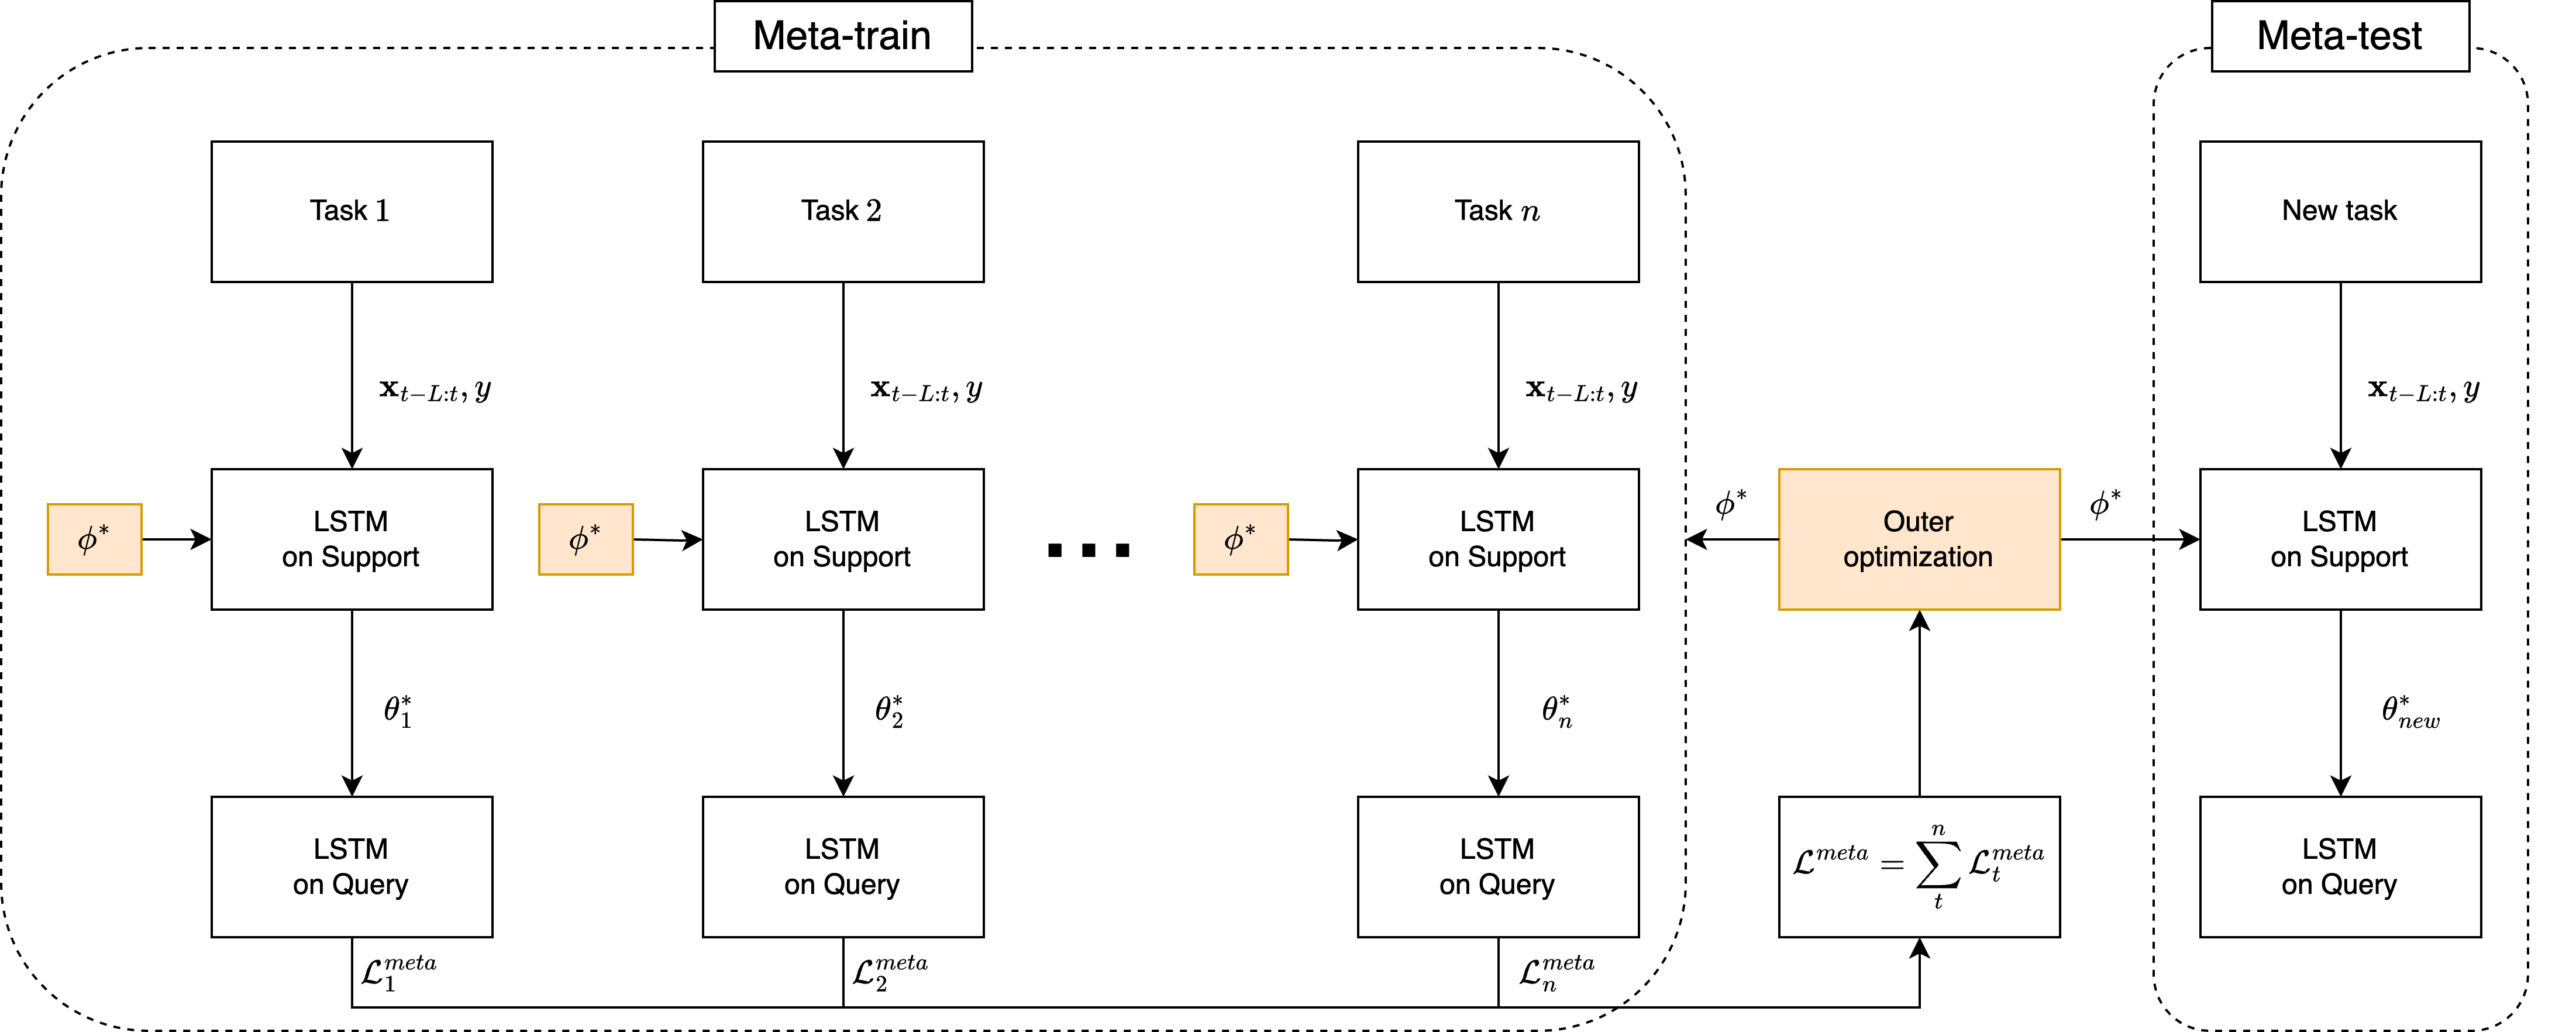
\includegraphics[width=\textwidth]{figs/meta.png}
    \caption{The flow of meta-training and meta-testing on multi-fx dataset.}
    \label{fig:flow}
\end{figure}

\subsection{Data preparation}
\label{subsec:method_data}

\verb|Temporal-ML| bases on ML algorithms to train the model. Therefore, the data must be reorganized so that the ML algorithms can work. In case the data includes many different datasets belonging to the same field, each dataset will be considered a task. The goal of using multiple datasets of the same domain is to utilize the corelation between them as indicated in study \cite{overreactioncontrarian, mech1993portfolio}. In case the data includes a single dataset, it is necessary to divide this dataset into subsets corresponding to separate tasks. By this way, we aim to enhance the learning of information about external factor reflected in single dataset \cite{fama1970efficient}. In summary, the prepared dataset includes $n$ tasks: $\mathcal{D} = \left\{ \mathcal{D}_t \right\}_{t=1}^{n}$. The data at each task is divided into support and query sets: $\mathcal{D}_t = \left\{ \mathcal{D}_t^{support}, \mathcal{D}_t^{query} \right\}$.

\vspace{1mm}

A datapoint consists of a pair of values $(\mathbf{x}_{t-L:t}, y)$. In which, $\mathbf{x}_{t-L:t}$ includes $L$ historical values from timestamp $t$; $y\in \{0,1\}$ is the label, showing the decreasing or increasing trend of the data sample $x_{t+1}$ compared to $x_{t}$. Depending on each problem and the implementation, the elements in $\mathbf{x}_{t-L:t}$ can be a matrix or a vector. For example, consider stock data, $\mathbf{x}_{t-L:t}$ can contain $L$ vectors $\vec x_i = (\text{open, low, high, close})$ or can be a vector of close price values only.

\subsection{Temporal feature extraction}

Temporal feature extraction is performed using \verb|BiLSTM|. Specifically, since every datapoint in time-series data usually has a small number of attribute, each element in the matrix $\mathbf{x}_{t-L:t}$ (abbreviated as $\mathbf{x}$) is passed through a \verb|FullyConnected| layer (with a non-linear activation function) whose output is larger than the dimension of $\vec x_i, i\in[t-L, t]$ to obtain vector $\vec x'_i$ (equation \ref{eq:decompose}). Accordingly, the data characteristics are expressed deeper and clearer. These features are then passed through the \verb|BiLSTM| network (equation \ref{eq:feature_lstm}) to selectively extract long-term temporal dependencies ($\mathbf{h}_{BiLSTM}$). At the end, $\mathbf{h}_{BiLSTM}$ is passed through a classification head of the neural network (equation \ref{eq:clf}) to predict the label of $\mathbf{x}$.

\begin{align}
    \mathbf{x'} &= \mathbf{FullyConnected}\left( \mathbf{x} \right) \label{eq:decompose}\\
    \mathbf{h}_{BiLSTM} &= \mathbf{BiLSTM}\left( \mathbf{x'} \right) \label{eq:feature_lstm}\\
    \hat y &= \mathbf{FullyConnected}\left( \mathbf{h}_{BiLSTM} \right) \label{eq:clf}
\end{align}

\verb|BiLSTM| maintains cell-state values to selectively store temporal dependencies, as well as to mitigate the vanishing gradient problem during training. Therefore, it is well suited for solving time-series data problems. Compared to \verb|LSTM|, \verb|BiLSTM| is superior in capturing global context of a sequence as well as solving the problem of information forgetting when dealing with long sequences in \verb|LSTM|. This is because \verb|BiLSTM| can extract and synthesize information from both sides of the input sequence. In conclusion, \verb|BiLSTM| can capture the entire context with minimal information loss for long sequences. In the context of the movement prediction problem of aperiodic time-series data, \verb|BiLSTM| is expected to successfully capture continuous value variation as well as not miss important information at distant inputs.

\subsection{Efficient model synthesis}

We use \verb|MAML| to train and aggregate the weights of the models of all tasks via the \verb|CrossEntropyLoss| (equation \ref{eq:loss}).

\begin{align}
    \mathcal{L}(\mathbf{y}, \hat{\mathbf{y}}) = \mathbb{E}\left[(\mathbf{y}\log{\hat{\mathbf{y}}}) + (1-\mathbf{y})\log{(1-\hat{\mathbf{y}})}\right]
    \label{eq:loss}
\end{align}

As mentioned in section \ref{subsec:ml}, parameter optimization in the ML approach is to solve the two equations \ref{eq:inner_opt} and \ref{eq:outer_opt} using optimization methods on the support set and query set. Specifically, the optimization process includes many global steps (outer optimization), performed on all tasks participating in training. Each global step includes many local steps (inner optimization) performed on each individual task. At global step $r$, the $e$th local optimization process on the support set of task $t$ proceeds as follows:

\begin{align}
    \begin{cases}
        \theta_t^{(0)} &= \phi_{r-1} \\
        \theta_t^{(e)} &= \theta_t^{(e-1)} - \alpha \nabla_{\theta} \mathcal{L}^{task}_t\left( \theta_t^{(e-1)}, \mathcal{D}_t^{support} \right)
    \end{cases}
    \label{eq:inner_sol}
\end{align} In which, $\phi_{r-1}$ is the result of the $r-1$ outer optimization process, $\alpha$ is the inner learning rate, $\mathcal{L}_t^{task}$ evaluates the use of $\theta_t^{(e-1)}$ on $\mathcal{D}_t^{support}$.

\vspace{1mm}

Next, the outer optimization process is performed by aggregating the losses on the query set of the tasks and optimizing on it (equation \ref{eq:outer_sol}).

\begin{align}
    \begin{cases}
        \phi_0 = \text{Random Initialization}\\
        \phi_r = \phi_{r-1} - \beta \nabla_{\phi} \sum_{t=1}^n{\mathcal{L}^{meta}_t \left( \theta_t(\phi), \mathcal{D}_t^{query} \right)}
    \end{cases}
    \label{eq:outer_sol}
\end{align} Where, $\beta$ is the outer learning rate, $\theta_t^*(\phi)$ is the local optimized weight obtained from equation \ref{eq:inner_sol}, $\mathcal{L}_t^{meta}$ evaluates the use of $\theta_t(\phi)$ on $\mathcal{D}_t^{query}$.

\vspace{1mm}

Assuming the algorithm runs $E$ steps in inner optimization, the derivative quantity at equation \ref{eq:outer_sol} is rewritten as follows (the notations of dataset are removed):

\begin{align}
    &\nabla_{\phi} \sum_{t=1}^n{\mathcal{L}^{meta}_t \left( \theta_t - \alpha \nabla_{\theta} \mathcal{L}^{task}_t\left( \theta_t \right) \right)}\\
    &= \sum_{t=1}^n{ \frac{\partial \mathcal{L}^{meta}_t\left(\theta_t^{(E)}\right)}{\partial \theta_t^{(E)}} \frac{\partial \theta_t^{(E)}}{\partial \phi}}\\
    &= \sum_{t=1}^n{ \nabla_{\theta} \mathcal{L}^{meta}_t\left(\theta_t^{(E)}\right) \prod_{j=0}^{E-1} {\left[\mathbb{I} - \alpha\nabla^2_{\theta}\mathcal{L}^{task}_{t}\left(\theta_t^{(j)}\right)\right]}}
    \label{eq:outer_grad}
\end{align}

As obtained in equation \ref{eq:outer_grad}, the outer optimization process requires large overhead in terms of memory and computation to train the model. As such, the number of computational steps to find $\theta^*$ needs to be limited. In practice, methods using ML \cite{chen2018federated, fallah2020personalized, finn2017model, li2017meta, nguyen2022meta} often choose $E\in [1,5]$.

\vspace{1mm}

Under the view point of ensemble learning, the synthesis process can be regarded as an efficient way to aggregate models. Thus, information from multiple data sources is efficiently aggregated. The model can then capture the correlations between different datasets. Moreover, by dividing a dataset into multiple sequences, we ensure that the global model can learn temporal feature from entire dataset, reducing the problem of information forgetting in \verb|BiLSTM|.

\section{Numerical experiment}

\subsection{Dataset}

Foreign exchange in particular and financial indices in general are typical data types for aperiodic time-series data. Therefore, we choose this type of data to test the model. Specifically, we configure two datasets using foreign exchange data. \verb|USD/JPY| dataset consists of only data of the exchange rate between US dollar and Japanese yen. The data is sampled hourly from 2000 to 2024, including 4 attributes: \textit{open, low, high, and close price}. By carefully examining the transaction history as well as effectively aggregating data characteristics, we expect to forecast the movement of price without utilizing external information. \verb|multi-fx| dataset consists of 60 currency pairs made of 18 countries: Australia, Canada, Switzerland, Denmark, EU, United Kingdom, Hong Kong, Iceland, Japan, Norway, New Zealand, Singapore, Sweden, Turkey, United States, Mexico, China, South Africa. The data has similar attributes to \verb|USD/JPY| and is sampled daily from 2014 to 2024. By integrating analysis of multiple sources of information in the domain of FX, we expect to obtain valuable analytical insights for the indicator of interest.

\vspace{1mm}

In addition, we use two periodic datasets: Electricity Transformer Temperature (\verb|ETT-m2|) \cite{zhou2021informer} and Weather (\verb|WTH|) \cite{Kolle}. \verb|ETT-m2| dataset consists of 7 attributes, measuring parameters of a transformer in a province of China every 15 minutes from July 2016 to July 2018. \verb|WTH| dataset consists of 12 attributes, recording the weather parameters at the Weather Station of the Max Planck Biogeochemistry Institute in Jena, Germany every 10 minutes in 2020. These two datasets exhibit very strong periodicity, which frequency decomposition-based methods have been very successful in predicting. Experiments on them provide a more comprehensive insight of the proposed method's capabilities.

\subsection{Metric}

Our study uses \textit{Accuracy, Precision, Recall}, and \textit{F1-score} to evaluate the proposed method. Suppose \verb|Temporal-ML| is evaluated on a dataset $\mathcal{D}$ consisting of $a$ attributes and divided into $n$ tasks. The evaluation is performed by letting the model predict the movement of each attribute with all attributes as input, then performing two aggregation steps: (1) - Aggregation on tasks; (2) - Aggregation on attributes. This evaluation process is designed based on study \cite{challu2023nhits}.

\vspace{1mm}

\textbf{Aggregation on tasks}. Consider metric $m$ when the model predicts any attribute $k$ ($1\leq k \leq a$). After predicting attribute $k$, we obtain $n$ values: $\{m^{(k)}_1,\dots,m^{(k)}_n\}$. The process of synthesizing metrics $m$ of $n$ tasks is performed as follows:

\begin{align}
    \bar{m}^{(k)} &= \frac{1}{n}\sum_{i=1}^n{m^{(k)}_i} \label{eq:mean_task}\\
    s^{(k)}_m &= \sqrt{\frac{1}{n} \sum_{i=1}^n{\left(m^{(k)}_i - \bar{m}^{(k)}\right)^2}} \label{eq:std_task}
\end{align}

\textbf{Aggregation on attributes}. The model predicts all $a$ attributes and obtains $a$ metrics: $\left\{ \left( \bar{m}^{(k)}\pm s^{(k)}_m \right) \right\}_{k=1}^a$. The process of synthesizing metric $m$ of $a$ attributes is as follows:

\begin{align}
    \bar{m} &= \frac{1}{a}\sum_{k=1}^a{\bar{m}^{(k)}} \label{eq:mean_att}\\
    s_m &= \sqrt{\frac{1}{a} \sum_{k=1}^a{\left(s^{(k)}_m\right)^2}} \label{eq:std:att}
\end{align}

\subsection{Experimental setup}

% setup baseline
This study uses \verb|NHITS| (AAAI 2023) as the baseline model. \verb|NHITS| uses the entire attributes to predict the next trend for an attribute in a dataset. The algorithm aims to decompose the frequency bands and combine them to predict the future. For \verb|USD/JPY|, \verb|ETT-m2|, and \verb|WTH| datasets, the data in each set is divided into a training set, a validation set, and a test set with a ratio of 6:2:2, respectively. For \verb|multi-fx| dataset, since \verb|NHITS| does not have a mechanism to aggregate models across different datasets, we repeat the training process (training, validation, testing on 60\%, 20\%, 20\% of the data, respectively) for each currency pair, then aggregate metrics across currency pairs to obtain the final evaluation. In addition, a random model is also used for comparison. This model generates predicted values of 0 and 1 according to a uniform distribution. The process of synthesizing metrics of this model is similar to \verb|NHITS|.

\vspace{1mm}

% setup our method
As mentioned in subsection \ref{subsec:method_data}, to use ML, the datasets need to be structured into separate tasks. In each task, the support set accounts for 20\% of the data, the query set accounts for 80\% of the data. The statistics of tasks in datasets are presented in Table \ref{tab:stat_}. In which, the ratio of tasks used for meta training, validation, and testing is 50:25:25. The details of dividing tasks is presented in Appendix \ref{app:preprocessing}.

\vspace{1mm}

\begin{table}[h]
    \centering
    \caption{Statistics on datasets.}
    \label{tab:stat_}
    % \resizebox{\columnwidth}{!}{}
    \begin{tblr}{
        cells = {c},
        hline{1,6} = {-}{0.08em},
        hline{2} = {-}{},
        }
        Dataset                      & \#Attribute & \#Task & \#Sample    & \#Sample/Task    \\
        USD/JPY                      & 4           & 60     & 150,175     & 2,503          \\
        multi-fx                     & 4           & 120    & 154,440     & 1,287          \\
        ETT-m2                       & 7           & 48     & 69,680      & 1,452          \\
        WTH                          & 12          & 40     & 35,064      & 877            
    \end{tblr}
\end{table}

% normalization
Before data is fed to model, it is normalized by \verb|z-score|. Specifically, training data is used to compute mean and standard deviation of each attribute. Then, these values are used to normalize validation and testing data. All models are trained on training set and validated on validation set. The best model is selected based on the performance on validation set. The final performance on testing set is reported. The details of tuning process is presented in Appendix \ref{app:tuning}.

\subsection{Ablation study}
\label{subsec:ab_exp}

We evaluate each component in \verb|Temporal-ML| by removing or replacing it and compare the results to the original algorithm. Specifically, we conduct experiments on two groups of algorithms: (1) - Model with \verb|BiLSTM| replaced; (2) - Model without ML. Regarding the evaluation of these models, ML-based models are evaluated as \verb|Temporal-ML|, the remaining models are evaluated as \verb|NHITS|. The details of model architectures are presented in Appendix \ref{app:ab_model}.

\vspace{1mm}

\textbf{Model with} \verb|BiLSTM| \textbf{replaced}. In this group, we replace \verb|BiLSTM| with \verb|BiLSTM+CNN|, \verb|Transformers|. The goal of replacing \verb|BiLSTM| with \verb|BiLSTM+CNN| is to test the local feature extraction ability of the extractor. In order to do so, we concatenate the features of \verb|BiLSTM| and \verb|CNN| then performing classification. The purpose of using \verb|Transformers| is to compare the performance of attention mechanism to \verb|BiLSTM| on aperiodic time-series data.

\vspace{1mm}

\textbf{Model without ML}. To study the impact of \verb|MAML| as well as optimization-based ML algorithms on \verb|Temporal-ML|, we remove this component and only use the pure feature extraction methods introduced above: \verb|BiLSTM|, \verb|BiLSTM+CNN|, \verb|Transformers|. Through this, the ability to effectively synthesize information from multiple sources of \verb|MAML| in aperiodic time-series data will be clarified. The dataset which contains information from multiple sources is \verb|multi-fx| dataset. Thus, we only experiment on this dataset.

\section{Result \& Discussion}

\subsection{Main result}

The main results of this work are shown in Table \ref{tab:mine_nhits}. Accordingly, our proposed method outperforms \verb|NHITS| on all metrics on two aperiodic datasets. On periodic datasets, our model achieves a competitive results compared to the baseline model. Specifically, for \verb|USD/JPY| and \verb|multi-fx| dataset, \verb|Temporal-ML| improves from 12\% to 14\% on metrics compared to the \verb|NHITS|. On the other hand, for periodic datasets, the accuracy of \verb|Temporal-ML| is 1\% lower, and the remaining metrics are 4-5\% lower than \verb|NHITS| on \verb|ETT-m2| data. For strongly cyclical data such as \verb|WTH|, our algorithm outperforms \verb|NHITS| by about 1\%. In addition, \verb|Temporal-ML| also achieves 1-3\% lower dispersion on metrics than \verb|NHITS| when operating in multi-source data context.

\vspace{1mm}

\begin{table*}[H]
    \centering
    \caption{Classification results (\%) of Temporal-ML and NHITS on aperiodic (USD/JPY, multi-fx) and periodic (ETT-m2, WTH) datasets. Best results per metrics are boldfaced. (\mbox{*}): Our method.}
    \label{tab:mine_nhits}
    \begin{tabular}{c|c|cccc}
        \toprule
        \multicolumn{1}{c}{}                &                                & $accuracy$              & $precision$             & $recall$                & $F1-score$                 \\
        \hline
        \multirow{2}{*}{USD/JPY}     		& NHITS                   & $58.46$                 & $58.24$                 & $57.65$                 & $55.82$            \\
                                            & Temporal-ML\mbox{*}     & $\mathbf{70.33\pm1.69}$ & $\mathbf{70.73\pm1.82}$ & $\mathbf{70.26\pm1.93}$ & $\mathbf{69.28\pm2.50}$    \\
                                            % & Ours(\verb|BiLSTM+CNN|)  & $68.75\pm1.78$          & $69.15\pm1.55$          & $68.73\pm1.77$          & $69.14\pm2.17$             \\
        \hline
        \multirow{2}{*}{multi-fx}           & NHITS                   & $53.51\pm5.02$          & $53.90\pm7.68$          & $53.64\pm4.05$          & $50.20\pm7.35$              \\
                                            & Temporal-ML\mbox{*}     & $\mathbf{66.26\pm7.45}$ & $\mathbf{67.08\pm8.97}$ & $\mathbf{65.76\pm7.79}$ & $\mathbf{64.06\pm10.00}$   \\
                                            % & Ours(\verb|BiLSTM+CNN|)  & $66.08\pm8.19$          & $66.56\pm9.23$          & $65.41\pm8.66$          & $63.78\pm10.83$            \\
        \hline
        \multirow{2}{*}{ETT-m2}             & NHITS                   & $\mathbf{71.88}$        & $\mathbf{66.86}$        & $\mathbf{62.49}$        & $\mathbf{62.69}$   \\
                                            & Temporal-ML\mbox{*}     & $71.14\pm9.13$          & $62.21\pm7.51$          & $58.75\pm5.30$          & $57.61\pm6.74$             \\
                                            % & Ours(\verb|BiLSTM+CNN|)  & $71.40\pm9.10$          & $63.25\pm8.82$          & $60.22\pm8.42$          & $59.43\pm9.24$             \\
        \hline
        \multirow{2}{*}{WTH}		        & NHITS                   & $74.18$                 & $68.05$                 & $65.04$                 & $65.40$             \\
                                            & Temporal-ML\mbox{*}     & $\mathbf{74.97\pm2.63}$ & $\mathbf{69.13\pm3.44}$ & $\mathbf{65.98\pm3.96}$ & $\mathbf{66.00\pm3.80}$    \\
                                            % & Ours(\verb|BiLSTM+CNN|)  & $74.41\pm2.71$          & $68.17\pm4.60$          & $65.50\pm4.82$          & $65.63\pm4.47$             \\
        \bottomrule
        \end{tabular}
\end{table*}

In Table \ref{tab:mine_nhits}, the results are aggregated as the average of all features, so they are highly representative. However, these results lack detail in the evaluation. Therefore, we analyze the results of the algorithms on each attribute of the aperiodic datasets in Table \ref{tab:mine_nhits_att}. Accordingly, when \verb|NHITS| predicts the attributes \textit{hight, low, close price} on both datasets, the results are only very close to the random prediction model. This shows that prediction on aperiodic data is really difficult. On the other hand, \verb|Temporal-ML| fails to predict \textit{low price} of \verb|USD/JPY| (accuracy approaching random prediction level). All other features of both datasets achieve high convergence and are significantly higher than \verb|NHITS|. This demonstrates the superiority of the proposed algorithm on aperiodic data.

\vspace{1mm}

\begin{table*}[H]
    \centering
    \caption{Accuracy (\%) of Temporal-ML and NHITS on each attribute of USD/JPY and multi-fx dataset. Best results per metrics are boldfaced. (\mbox{*}): Our method.}
    \label{tab:mine_nhits_att}
    \begin{tabular}{c|c|cccc}
        \toprule
        \multicolumn{1}{c}{}                &                                & $Open$                  & $High$                  & $Low$                   & $Close$                     \\
        \hline
        \multirow{3}{*}{USD/JPY}            & Random                         & $49.91$                 & $49.91$                 & $50.33$                 & $50.66$                     \\
                                            & NHITS                   & $75.03$                 & $53.74$                 & $51.57$                 & $53.50$                     \\
                                            & Temporal-ML\mbox{*}     & $\mathbf{93.06\pm1.36}$ & $\mathbf{68.87\pm1.53}$ & $\mathbf{51.01\pm1.58}$ & $\mathbf{68.37\pm2.16}$     \\
        \hline
        \multirow{3}{*}{multi-fx}           & Random                         & $49.92\pm2.19$          & $49.93\pm2.22$          & $49.94\pm2.17$          & $49.85\pm2.13$              \\
                                            & NHITS                   & $58.36\pm7.13$          & $50.66\pm4.28$          & $51.17\pm3.21$          & $53.84\pm4.60$              \\
                                            & Temporal-ML\mbox{*}     & $\mathbf{78.13\pm6.33}$ & $\mathbf{62.74\pm3.30}$ & $\mathbf{58.28\pm3.86}$ & $\mathbf{65.88\pm12.49}$    \\
        \bottomrule
        \end{tabular}
\end{table*}

To clarify the capabilities of \verb|Temporal-ML|, based on the main results and the results obtained from ablation experiments (subsection \ref{subsec:ab_exp}), we analyze the proposed algorithm on two aspects: (1) - Temporal feature extraction ability; (2) - Models' parameters aggregation ability.

\subsection{Temporal feature extraction ability}

From the tables \ref{tab:mine_nhits} and \ref{tab:mine_nhits_att}, it is not difficult to see that the temporal feature extraction ability of \verb|Temporal-ML| is much better than that of \verb|NHITS|. Indeed, the feature extraction and synthesis process of \verb|NHITS| shows that this method is trying to simulate the frequency resolution process of Fourier transform. The frequency band features are the most important information for periodic data. Therefore, the predictions of \verb|NHITS| can easily achieve high accuracy on this type of data. However, it is very difficult to achieve frequency resolution on aperiodic data. Furthermore, the time-series data, although filtered through multiple stacks to extract low-to-high frequency bands, the filtering techniques used in the network are extremely simple (using only \verb|FullyConnected| with nonlinear activation functions and \verb|Pooling| layers). This is what makes \verb|NHITS| a major obstacle on \verb|multi-fx|, \verb|USD/JPY| datasets and aperiodic data in general.

\vspace{1mm}

To better understand the capabilities of \verb|BiLSTM|, we performed an ablation study on this component of \verb|Temporal-ML| and presented the results in Table \ref{tab:ab_lstm}. Accordingly, when \verb|BiLSTM| is replaced by other components (\verb|BiLSTM+CNN|, \verb|Transformers|) for temporal feature extraction, the results on all four metrics of most datasets are lower than those obtained by \verb|Temporal-ML|. Specifically, on two aperiodic datasets (\verb|USD/JPY| and \verb|multi-fx|), the algorithms using \verb|BiLSTM+CNN| and \verb|Transformers| to extract features give 2-10\% lower in prediction ability than \verb|Temporal-ML|. On periodic data, \verb|MAML(Transformer)| still gives much lower results than \verb|Temporal-ML|. However, \verb|MAML(BiLSTM+CNN)| gives results that are almost asymptotically close to the proposed algorithm. On all four datasets, the standard deviation of the metrics of the proposed algorithm is generally 1-5\% smaller than the remaining algorithms.

\vspace{1mm}

\begin{table*}[H]
    \centering
    \caption{Classification results (\%) of Temporal-ML and models with BiLSTM replaced. Best results per metrics are boldfaced. (\mbox{*}): Our method.}
    \label{tab:ab_lstm}
    \begin{tabular}{c|c|cccc} 
        \toprule
        \multicolumn{1}{c}{}      &                                          & $accuracy$               & $precision$              & $recall$                 & $F1-score$                \\ 
        \hline
        \multirow{3}{*}{USD/JPY} & Temporal-ML\mbox{*}         & $\mathbf{70.33\pm1.69}$  & $\mathbf{70.73\pm1.82}$  & $\mathbf{70.26\pm1.93}$  & $\mathbf{69.28\pm2.50}$   \\
                                        & MAML(BiLSTM+CNN)     & $68.75\pm1.78$           & $69.15\pm1.55$           & $68.73\pm1.77$           & $69.14\pm2.17$            \\
                                        & MAML(Transformers)   & $60.67\pm4.09$           & $59.74\pm6.24$           & $59.32\pm3.79$           & $53.15\pm6.19$            \\ 
        \hline
        \multirow{3}{*}{multi-fx}& Temporal-ML\mbox{*}         & $\mathbf{66.26\pm7.45}$  & $\mathbf{67.08\pm8.97}$  & $\mathbf{65.76\pm7.79}$  & $\mathbf{64.06\pm10.00}$  \\
                                        & MAML(BiLSTM+CNN)     & $66.08\pm8.19$           & $66.56\pm9.23$           & $65.41\pm8.66$           & $63.78\pm10.83$           \\
                                        & MAML(Transformers)   & $56.03\pm6.08$           & $56.32\pm6.01$           & $55.63\pm5.01$           & $52.33\pm7.08$            \\ 
        \hline
        \multirow{3}{*}{ETT-m2}  & Temporal-ML\mbox{*}         & $71.14\pm9.13$           & $62.21\pm7.51$           & $58.75\pm5.30$           & $57.61\pm6.74$            \\
                                        & MAML(BiLSTM+CNN)     & $\mathbf{71.40\pm9.10}$  & $\mathbf{63.25\pm8.82}$  & $\mathbf{60.22\pm8.42}$  & $\mathbf{59.43\pm9.24}$   \\
                                        & MAML(Transformers)   & $68.69\pm8.85$           & $58.54\pm4.38$           & $57.85\pm4.71$           & $57.07\pm5.14$            \\ 
        \hline
        \multirow{3}{*}{WTH}     & Temporal-ML\mbox{*}         & $\mathbf{74.97\pm2.63}$  & $\mathbf{69.13\pm3.44}$  & $\mathbf{65.98\pm3.96}$  & $\mathbf{66.00\pm3.80}$   \\
                                        & MAML(BiLSTM+CNN)     & $74.41\pm2.71$           & $68.17\pm4.60$           & $65.50\pm4.82$           & $65.63\pm4.47$            \\
                                        & MAML(Transformers)   & $72.28\pm3.06$           & $62.35\pm8.73$           & $60.90\pm4.97$           & $58.65\pm4.72$            \\
        \bottomrule
    \end{tabular}
\end{table*}

According to this result, it can be seen that using \verb|BiLSTM| brings high and stable results in the prediction process. Using networks such as \verb|CNN|, \verb|Transformers| not only create negative improvements but also disturbs the learning process or reduces the efficiency of the whole model. For using \verb|BiLSTM+CNN|, the learning process is disturbed because \verb|BiLSTM| itself has selected effective time dependencies during the extraction process while \verb|CNN| only extracts features but does not select. This leads to the instability of \verb|BiLSTM+CNN|'s features. If \verb|CNN| extracts good features, the network will perform well (e.g., metrics on \verb|ETT-m2|). On the contrary, the network will perform worse than using only \verb|BiLSTM| (e.g., metrics on \verb|USD/JPY|, \verb|multi-fx|, \verb|WTH|).

\vspace{1mm}

With the above analysis, we conclude that \verb|BiLSTM| is not only a suitable choice for exploring the variability of aperiodic time-series data but also a suitable algorithm to combine with ML algorithms when working on time-series data in general. By using \Verb|BiLSTM|, we have effectively extracted market fluctuations and predicted the future.

\subsection{Models' parameters aggregation ability}

In the process of synthesizing features to make the final prediction, \verb|NHITS| only uses simple addition and subtraction. This makes sense in the context of synthesizing information based on the frequency bands extracted from the input data. Indeed, data related to weather, demand for airplanes or electricity show very strong periodic characteristics because weather and human consumption behavior, although they may vary over time, still show a very clear seasonality (e.g., cold weather in winter, high demand for airplanes during holidays). Therefore, the frequency of this type of data is a good feature and can be easily extracted. After decomposing the input data into frequency bands, we can simply synthesize them to be able to predict the future. In addition, synthesizing the frequency bands by an addition can be considered very simple compared to current deep learning algorithms, which work on the hidden feature space of the data. Therefore, the synthesis process of \verb|NHITS| on aperiodic data encounters many difficulties because the input information for the process is not good and the synthesis method is ineffective. Consequently, it can be seen that aperiodic time-series data becomes a fatal weakness for \verb|NHITS| and frequency decomposition-based methods in general.

\vspace{1mm}

Dealing with the complexity of non-periodic data requires a complex structure that can efficiently aggregate features. As mentioned in the Introduction, analyzing and synthesizing information from multiple data sources in the same domain can provide useful information for predicting metrics of interest. \verb|Temporal-ML| with the ability to synthesize information based on the optimization process of ML algorithms, allows the model to capture multi-dimensional information from different data sources, which can enhance the effectiveness of predictions.

\vspace{1mm}

To evaluate the capabilities of ML algorithms, we remove this component from the proposed method and then run experiments to compare with the original results. We use ML algorithms for the purpose of synthesizing multi-source information. Therefore, comparisons are only performed on the \verb|multi-fx| dataset because this dataset contains several sub-datasets from different sources, which helps to accurately evaluate the information synthesis capability. The results are summarized in Table \ref{tab:ab_ml}. Accordingly, with the information synthesis capability, \verb|Temporal-ML| achieves 2-12\% higher in all metrics than algorithms that do not use ML in testing process. In addition, the dispersion of the metrics is also lower from 1-7\%, proving that the difference in the task prediction process is much better than the remaining algorithms.

\vspace{1mm}

\begin{table*}[H]
    \centering
    \caption{Classification results (\%) of Temporal-ML and models without MAML on multi-fx dataset. Best results per metrics are boldfaced. (\mbox{*}): Our method.}
    \label{tab:ab_ml}
    \begin{tabular}{c|cccc} 
    \toprule
                                & $accuracy$              & $precision$             & $recall$                & $F1-score$                \\ 
    \hline
    Temporal-ML\mbox{*}  & $\mathbf{66.26\pm7.45}$ & $\mathbf{67.08\pm8.97}$ & $\mathbf{65.76\pm7.79}$ & $\mathbf{64.06\pm10.00}$  \\
    BiLSTM               & $63.88\pm9.00$          & $64.18\pm13.39$         & $63.66\pm9.13$          & $60.07\pm13.09$           \\
    BiLSTM+CNN           & $62.23\pm8.63$          & $62.89\pm9.76$          & $62.20\pm8.34$          & $59.91\pm10.97$           \\
    Transformers         & $58.44\pm9.15$          & $56.71\pm15.10$         & $58.22\pm8.84$          & $52.22\pm13.12$           \\
    \bottomrule
    \end{tabular}
\end{table*}

The better performance of \verb|Temporal-ML| on \verb|multi-fx| is understandable because all the remaining methods in the \ref{tab:ab_ml} table do not have the ability to synthesize information like the proposed algorithm, but rely entirely on past data to predict the future. Therefore, not only \verb|BiLSTM|, \verb|BiLSTM+CNN| but also \verb|Transformers| cannot take advantage of the correlation between data sources.

Therefore, it can be seen that, the use of optimization-based ML algorithms in information synthesis is completely reasonable because it successfully takes advantage of the correlation between data sets and achieves high accuracy without requiring too much data as in the single-source context.

\section{Conclusion}

Problems on aperiodic time-series data pose a great challenge to current machine learning models because this data depends on both transaction history and external factors such as economic and political situations; the variance of the data changes continuously; the aperiodicity of the data is very strong. By utilizing the time constraint extraction capability of \verb|BiLSTM| and the efficient parameter synthesis capability of \verb|MAML|, we propose the \verb|Temporal-ML| algorithm with the ability to extract hidden time features as well as synthesize information from multi-source data. Based on experiments, in the process of solving the next trend prediction problem, the proposed method achieves high efficiency on two aperiodic data sets (\verb|USD/JPY| and \verb|multi-fx|) and equivalent efficiency on periodic data sets (\verb|ETT-m2| and \verb|WTH|) compared to \verb|NHITS| - a frequency decomposition based approach. In addition, by performing an ablation study, we demonstrate the superior of \verb|BiLSTM| in extracting temporal feature compared to \verb|CNN|, \verb|Transformers| and the effectiveness of \verb|MAML| in synthesizing information from multi-source data. The results of this study are expected to be a good foundation for future research on time-series data.

Our experiment only illustrates a typical case of efficient model synthesis. In the future, by using different ML algorithms such as \verb|Meta-SGD| \cite{li2017meta}, \verb|Reptile| \cite{nichol2018first}, \verb|iMAML| \cite{rajeswaran2019meta}, it is possible to generate new models with higher accuracy. On the other hand, it is possible to extend this method to solve long-horizon prediction problems. Indeed, by changing the output and error of the model, it is possible to solve these problems. However, the architecture of the sub-models needs to be re-examined to better suit the new problem.

\appendix

\section{Data preprocessing}
\label{app:preprocessing}

\subsection{Task-based preprocessing}

Since the datasets are all time-series, the training data should not reveal any information about the future. Therefore, we divide every currency pair in \verb|multi-fx| into 2 tasks, resulting in 120 tasks. The first parts of every pair are used for meta-training. The second parts of them are used for meta validating and meta testing with the ratio of 50:50. The remaining datasets are is divided into periods of time, each corresponding to a task.

\vspace{1mm}

The \verb|z-score| preprocessing is performed on training data to obtain mean and standard deviation values. These values are used to normalize the data of validation set and test set.

\subsection{Fairness in evaluation}

Let $m$ be the number of data samples in each task, the total data of training, validating, and testing is: $mn$. For \verb|NHITS|, the model is trained, validated, and tested on 60\%, 20\%, 20\% of the data, respectively:

\begin{align}
    \text{Train: } &0.6mn\\
    \text{Validation: } &0.2mn\\
    \text{Testing: } &0.2mn
\end{align}

For \verb|Temporal-ML|, the knowledge enrichment process for the model uses the entire training data and the support set of the testing/validation data. The testing/validation process is performed on the query set:

\begin{align}
    \text{Train: } &0.5mn + 2\times 20\%(0.25mn) = 0.6mn\\
    \text{Validation: } &80\% (0.25mn)  =0.2mn\\
    \text{Testing: } &80\% (0.25mn)  =0.2mn
\end{align}

Therefore, with the above data division, we achieve fairness in the number of data samples during testing.

\section{Hyperparameter tuning}
\label{app:tuning}

\subsection{Temporal-ML}

In our implementation, we use a \verb|FullyConnected| layer of 16 units with a \verb|ReLU| activation function to represent deeper and more explicit features. This feature is then passed to a \verb|BiLSTM| block. The \verb|BiLSTM| block consists of 32 hidden units, two last outputs of which are concatenated to form a final vector. This vector is then passed through a binary classification layer with a \verb|Sigmoid| activation function.

\vspace{1mm}

The fine-tuning process of ML algorithms involves many hyper-parameters such as inner batch size, outer batch size, inner training step, outer training step, etc. To make fine-tuning easy, we fix most of the parameters and only fine-tune the size of lookback window, inner and outer learning rate. Details are presented in Table \ref{tab:our_finetune}.

\begin{table}[H]
    \centering
    \caption{Search space for fine-tuning our method.}
    \label{tab:our_finetune}
    % \resizebox{\columnwidth}{!}{}
    \begin{tabular}{ll} 
        \toprule
        \multicolumn{1}{c}{Hyper-parameter} & \multicolumn{1}{c}{Seach space}   \\ 
        \hline
        Inner batch size (samples/batch)    & \{32\}                            \\
        Inner training step                 & \{3\}                             \\
        Outer batch size (tasks/batch)      & \{5\}                             \\
        Outer training step                 & \{100\}                           \\ 
        \hline
        Lookback window                     & \{10, 20, 30\}                    \\
        Inner learning rate                 & \{0.001, 0.00325, 0.0055, 0.00775, 0.01\}\\
        Outer learning rate                 & \{0.001, 0.00325, 0.0055, 0.00775, 0.01\}\\
        \bottomrule
    \end{tabular}
\end{table}

\subsection{NHITS}

We rely on study \cite{challu2023nhits} to define the search space (Table \ref{tab:nhits_finetune}) for parameter fine-tuning. For parameters not mentioned in the table, we use the default values of the \verb|NHITS| implementation in \verb|NeuralForecast| library \cite{neuralforecast}. The best results of fine-tuning process are selected and reported in this study.

\begin{table}[H]
    \centering
    \caption{Search space for fine-tuning NHITS.}
    \label{tab:nhits_finetune}
    % \resizebox{\columnwidth}{!}{}
    \begin{tabular}{ll} 
        \toprule
        \multicolumn{1}{c}{Hyper-parameter} & \multicolumn{1}{c}{Seach space}                              \\ 
        \hline
        Random seed                         & \{1\}                                                        \\
        Number of stacks                    & \{3\}                                                        \\
        Number of blocks in each stack      & \{1\}                                                        \\
        Activation function                 & \{ReLU\}                                                     \\
        Batch size                          & \{256\}                                                      \\
        Epoch                               & \{500\}                                                      \\ 
        \hline
        Lookback window                     & \{10, 20, 30\}                                                \\
        Pooling kernel                      & \{[2,2,2], [4,4,4], [8,8,8], [8,4,1], [16,8,1]\}           \\
        Stacks' coefficients                & \{[168,24,1], [24,12,1], [180,60,1],[40,20,1], [64,8,1]\}  \\
        Number of MLP layers                & \{1,2\}                                                      \\
        Learning rate                       & \{0.001, 0.00325, 0.0055, 0.00775, 0.01\}                          \\
        \bottomrule
        \end{tabular}
\end{table}

\section{Model architecture in ablation study}
\label{app:ab_model}

\verb|BiLSTM+CNN| model includes two parts: \verb|BiLSTM| and \verb|CNN|. The \verb|BiLSTM| part has the similar architecture with the one used in \verb|Temporal-ML|. The \verb|CNN| part consists of two \verb|Convolution1D| layers with \verb|ReLU| as activation function and the number of filters are 32 and 64, respectively. Each of convolution layer is followed by a \verb|MaxPooling| layer with the kernel size of 2. Next, the output of \verb|CNN| part is flatten and concatenated with the output of the \verb|BiLSTM| part. The concatenated is then passed through a classification head with \verb|Sigmoid| activation function.

\vspace{1mm}

\verb|Transformer| model is composed of two encoders. Each encoder uses three attention heads, and the key vector dimension is 256. The \verb|FeedForward| part of the encoder uses two \verb|Convolution1D| layers and one \verb|LayerNormalization|. After stacking the two encoder layers, the feature matrix is passed through a \verb|Flatten| layer and then fed into the classification head.

\printcredits

% \clearpage

%% Loading bibliography style file
%\bibliographystyle{model1-num-names}
\bibliographystyle{cas-model2-names}

% Loading bibliography database
\bibliography{cas-refs}

\end{document}

